%%
% BIThesis 研究生学位论文模板 The BIThesis Template for Graduate Thesis
% This file has no copyright assigned and is placed in the Public Domain.
%%

\chapter{基于几何结构约束的矿井巷道建图方法}



\label{chap:intro-ch3}
\tikzset{
  ch3box/.style={draw, rounded corners=3pt, thick, align=center, minimum height=8mm, minimum width=24mm, font=\small, fill=blue!8},
  ch3data/.style={draw, rounded corners=3pt, thick, align=center, minimum height=8mm, minimum width=24mm, font=\small, fill=green!10},
  ch3core/.style={draw, rounded corners=3pt, thick, align=center, minimum height=8mm, minimum width=26mm, font=\small, fill=orange!12},
  ch3aux/.style={draw, rounded corners=3pt, thick, align=center, minimum height=8mm, minimum width=26mm, font=\small, fill=purple!10},
  ch3solve/.style={draw, rounded corners=3pt, thick, align=center, minimum height=9mm, minimum width=28mm, font=\small\bfseries, fill=red!10},
  ch3arr/.style={-{Latex[length=2.5mm]}, thick},
  ch3darr/.style={-{Latex[length=2.5mm]}, thick, dashed},
  ch3node/.style={circle, draw, thick, inner sep=1.4pt, fill=white},
  ch3sel/.style={circle, draw, thick, inner sep=1.6pt, fill=black},
  ch3lab/.style={font=\small}
}
\section{引言}
矿井巷道环境狭长且结构重复，基于局部配准或里程计累积的建图方法容易在长距离运行中产生误差累积和轨迹漂移，导致地图全局一致性不足。尤其在缺少稳定回环约束时，传统后端优化难以充分利用巷道中的几何结构信息。因此，需要将全局几何先验与局部平面观测有效引入位姿图优化过程。

针对上述问题，本章提出一种基于几何结构约束的矿井巷道位姿图建图方法，整体流程如图 3.1 所示。
[此处插入图 3.1 基于几何结构约束的矿井巷道建图总体框架图]

\begin{figure}[htbp]
    \centering
    \begin{tikzpicture}[node distance=8mm and 8mm, scale=0.95, every node/.style={transform shape}]
        \node[ch3data] (pcd) {离线点云帧\\PCD 文件};
        \node[ch3data, right=of pcd] (odom) {外部里程计\\离线位姿文件};
        \node[ch3data, right=of odom] (planes) {地面与侧壁\\平面观测提取};

        \node[ch3box, below=12mm of odom] (assoc) {时间关联与\\关键帧筛选};
        \node[ch3core, left=18mm of assoc] (graph) {基础位姿图\\节点与里程计边};
        \node[ch3core, right=18mm of assoc] (global) {全局几何先验\\长度约束 + 角度约束};
        \node[ch3aux, below=10mm of assoc] (local) {局部几何辅助约束\\地面约束 + 侧壁约束};
        \node[ch3solve, below=12mm of local] (opt) {多因子图优化求解};
        \node[ch3box, below left=10mm and 14mm of opt] (traj) {优化关键帧轨迹};
        \node[ch3box, below right=10mm and 14mm of opt] (map) {全局一致地图};

        \draw[ch3arr] (pcd) -- (assoc);
        \draw[ch3arr] (odom) -- (assoc);
        \draw[ch3arr] (planes) -- (local);
        \draw[ch3arr] (assoc) -- (graph);
        \draw[ch3arr] (assoc) -- (global);
        \draw[ch3arr] (graph) -- (opt);
        \draw[ch3arr] (global) -- (opt);
        \draw[ch3arr] (local) -- (opt);
        \draw[ch3arr] (opt) -- (traj);
        \draw[ch3arr] (opt) -- (map);
    \end{tikzpicture}
    \caption{基于几何结构约束的矿井巷道建图总体框架图}
    \label{fig:overall_geom_mapping_framework}
\end{figure}

该方法以离线点云与外部里程计为基础，首先完成观测数据关联、关键帧筛选及基础位姿图构建；随后，将巷道场景中的全局长度先验和全局角度先验建模为核心几何约束，并与地面平面辅助约束、转弯区域侧壁方向辅助约束共同组成图优化模型；最后，通过多因子联合优化，有效抑制长距离建图过程中的误差累积，提升矿井巷道地图的全局一致性与结构准确性。
……\cite{Takahashi1996Structure,Xia2002Analysis,Jiang1989,Mao2000Motion,Feng1998}
\section{位姿图构建}

为将后续全局几何先验约束和局部平面观测约束统一纳入后端优化框架，本文首先构建矿井巷道场景下的位姿图模型。该模型以关键帧位姿作为状态节点，以相邻关键帧之间的相对位姿作为基础约束，从而为后续长度约束、角度约束及平面约束的引入提供统一的优化结构。位姿图构建流程如图~\ref{fig:pose_graph_pipeline} 所示。

\begin{figure}[htbp]
    \centering
    % \includegraphics[width=0.9\linewidth]{figures/pose_graph_pipeline.pdf}
    \begin{tikzpicture}[node distance=8mm and 10mm]
        \node[ch3data] (pcd2) {逐帧点云读取};
        \node[ch3data, below=10mm of pcd2] (odom2) {外部位姿读取};
        \node[ch3box, right=16mm of pcd2, yshift=-5mm] (assoc) {点云-位姿对应};
        \node[ch3box, right=of assoc] (kf) {关键帧判定};

        \node[ch3core, below=13mm of kf, xshift=-18mm] (nodeinit) {位姿节点初始化};
        \node[ch3core, right=of nodeinit] (relpose) {相对位姿计算};
        \node[ch3core, right=of relpose] (edge) {里程计边构建};
        \node[ch3solve, below=13mm of relpose] (posegraph) {位姿图形成};

        \draw[ch3arr] (pcd2.east) -- (assoc.west);
        \draw[ch3arr] (odom2.east) -- (assoc.west);
        \draw[ch3arr] (assoc) -- (kf);
        \draw[ch3arr] (kf) -- (nodeinit);
        \draw[ch3arr] (kf) -- (relpose);
        \draw[ch3arr] (nodeinit) -- (posegraph);
        \draw[ch3arr] (relpose) -- (edge);
        \draw[ch3arr] (edge) |- (posegraph);
    \end{tikzpicture}
    \caption{位姿图构建流程图}
    \label{fig:pose_graph_pipeline}
\end{figure}

\subsection{状态变量定义与观测数据关联}

在位姿图中，关键帧位姿是后端优化的基本状态变量。本文采用刚体变换群 $SE(3)$ 表示第 $i$ 个关键帧的位姿，即：
\begin{equation}
\mathbf{T}_i=
\begin{bmatrix}
\mathbf{R}_i & \mathbf{t}_i\\
\mathbf{0}^{\mathrm T} & 1
\end{bmatrix}
\in SE(3)
\end{equation}

其中，$\mathbf{R}_i \in SO(3)$ 为旋转矩阵，$\mathbf{t}_i \in \mathbb{R}^3$ 为平移向量。

本文使用的观测数据包括离线点云和外部位姿。其中，外部位姿由 FAST-GICP 通过相邻帧点云配准逐帧估计得到，用作位姿图构建的初始位姿。对每帧有效点云，直接读取其对应的外部位姿用于后续关键帧筛选与约束构建。

\subsection{关键帧筛选与里程计约束建模}

离线点云通常以较高频率连续采集，若将全部点云帧直接作为优化节点加入位姿图，会引入大量位姿变化较小的冗余节点。因此，本文采用关键帧筛选策略，根据当前帧与最近一个关键帧之间的位姿变化判断是否保留当前帧。

设当前帧位姿为 $\mathbf{T}_i$，最近一个关键帧位姿为 $\mathbf{T}_k$，则两者之间的相对位姿可表示为：
\begin{equation}
\Delta \mathbf{T}_{k,i}=\mathbf{T}_k^{-1}\mathbf{T}_i
\end{equation}

记 $\Delta \mathbf{T}_{k,i}$ 的平移部分和旋转部分分别为 $\Delta \mathbf{t}_{k,i}$ 和 $\Delta \mathbf{R}_{k,i}$，则平移增量和旋转增量可分别定义为：
\begin{equation}
\Delta s_{k,i}=\|\Delta \mathbf{t}_{k,i}\|_2
\end{equation}
\begin{equation}
\Delta \theta_{k,i}=\arccos\left(\frac{\mathrm{tr}(\Delta \mathbf{R}_{k,i})-1}{2}\right)
\end{equation}

其中，$\|\cdot\|_2$ 表示向量的 2 范数。当满足：
\begin{equation}
\Delta s_{k,i}>\tau_s \quad \text{or} \quad \Delta \theta_{k,i}>\tau_\theta
\end{equation}

时，将当前帧判定为新的关键帧，其中 $\tau_s$ 和 $\tau_\theta$ 分别为平移阈值和旋转阈值。通过该策略，可保留轨迹中的代表性位姿状态，并降低位姿图中的冗余约束。

对于选中的关键帧，本文以其外部位姿作为节点初值，并进一步利用相邻关键帧之间的相对位姿关系构建里程计约束。设相邻两个关键帧的位姿分别为 $\mathbf{T}_{i-1}$ 和 $\mathbf{T}_i$，则对应的相对位姿测量可表示为：
\begin{equation}
\mathbf{Z}_{i-1,i}=\mathbf{T}_{i-1}^{-1}\mathbf{T}_i
\end{equation}

其中，$\mathbf{Z}_{i-1,i}$ 表示从关键帧 $i-1$ 到关键帧 $i$ 的相对位姿测量。基于该测量，可在位姿图中构造连接相邻节点的二元约束边。设优化过程中节点当前估计位姿分别为 $\hat{\mathbf{T}}_{i-1}$ 和 $\hat{\mathbf{T}}_i$，则相应的里程计约束误差可写为：
\begin{equation}
\mathbf{e}_{i-1,i}
=
\mathrm{Log}
\left(
\mathbf{Z}_{i-1,i}^{-1}
\hat{\mathbf{T}}_{i-1}^{-1}
\hat{\mathbf{T}}_i
\right)
\end{equation}

其中，$\mathrm{Log}(\cdot)$ 表示从 $SE(3)$ 到李代数 $\mathfrak{se}(3)$ 的对数映射。对应的代价项可表示为：
\begin{equation}
J_{i-1,i}
=
\mathbf{e}_{i-1,i}^{\mathrm{T}}
\boldsymbol{\Omega}_{i-1,i}
\mathbf{e}_{i-1,i}
\end{equation}

其中，$\boldsymbol{\Omega}_{i-1,i}$ 为该约束的信息矩阵，用于描述测量的置信度。

此外，为保证优化参考坐标系的稳定性，本文对首帧节点施加锚点约束，以抑制位姿图整体漂移。由此，关键帧节点、相邻里程计约束以及首帧锚定约束共同构成位姿图的基础拓扑结构，如图~\ref{fig:base_pose_graph} 所示。

\begin{figure}[htbp]
    \centering
    % \includegraphics[width=0.85\linewidth]{figures/base_pose_graph.pdf}
    \begin{tikzpicture}[x=1.8cm,y=1cm]
        \node[draw, thick, rectangle, minimum width=0.9cm, minimum height=0.55cm, fill=gray!15] (anchor) at (-1.1,0) {锚点};
        \node[ch3node, label={[ch3lab]below:$\mathbf{T}_1$}] (k1) at (0,0) {};
        \node[ch3node, label={[ch3lab]below:$\mathbf{T}_2$}] (k2) at (1,0.25) {};
        \node[ch3node, label={[ch3lab]below:$\mathbf{T}_3$}] (k3) at (2,-0.1) {};
        \node[ch3node, label={[ch3lab]below:$\mathbf{T}_4$}] (k4) at (3,0.2) {};
        \node[ch3node, label={[ch3lab]below:$\mathbf{T}_5$}] (k5) at (4,-0.05) {};

        \draw[ch3darr] (anchor) -- node[ch3lab, above] {首帧锚定约束} (k1);
        \draw[ch3arr] (k1) -- node[ch3lab, above] {里程计边} (k2);
        \draw[ch3arr] (k2) -- (k3);
        \draw[ch3arr] (k3) -- (k4);
        \draw[ch3arr] (k4) -- (k5);
    \end{tikzpicture}
    \caption{基础位姿图结构示意图}
    \label{fig:base_pose_graph}
\end{figure}

综上，本文完成了关键帧状态初始化、关键帧筛选和基础里程计约束构建，为后续几何约束建模提供了位姿图基础。





\section{全局几何先验约束建模}

在完成基础位姿图构建后，仅依赖相邻关键帧之间的局部相对位姿约束仍难以从全局尺度上抑制长距离建图中的误差累积。针对矿井巷道中普遍存在的长度关系和转角关系，本文进一步引入长度先验约束和角度先验约束，对位姿图进行全局补充建模。全局几何先验约束建模示意如图~\ref{fig:global_geom_constraints} 所示。

\begin{figure}[htbp]
    \centering
    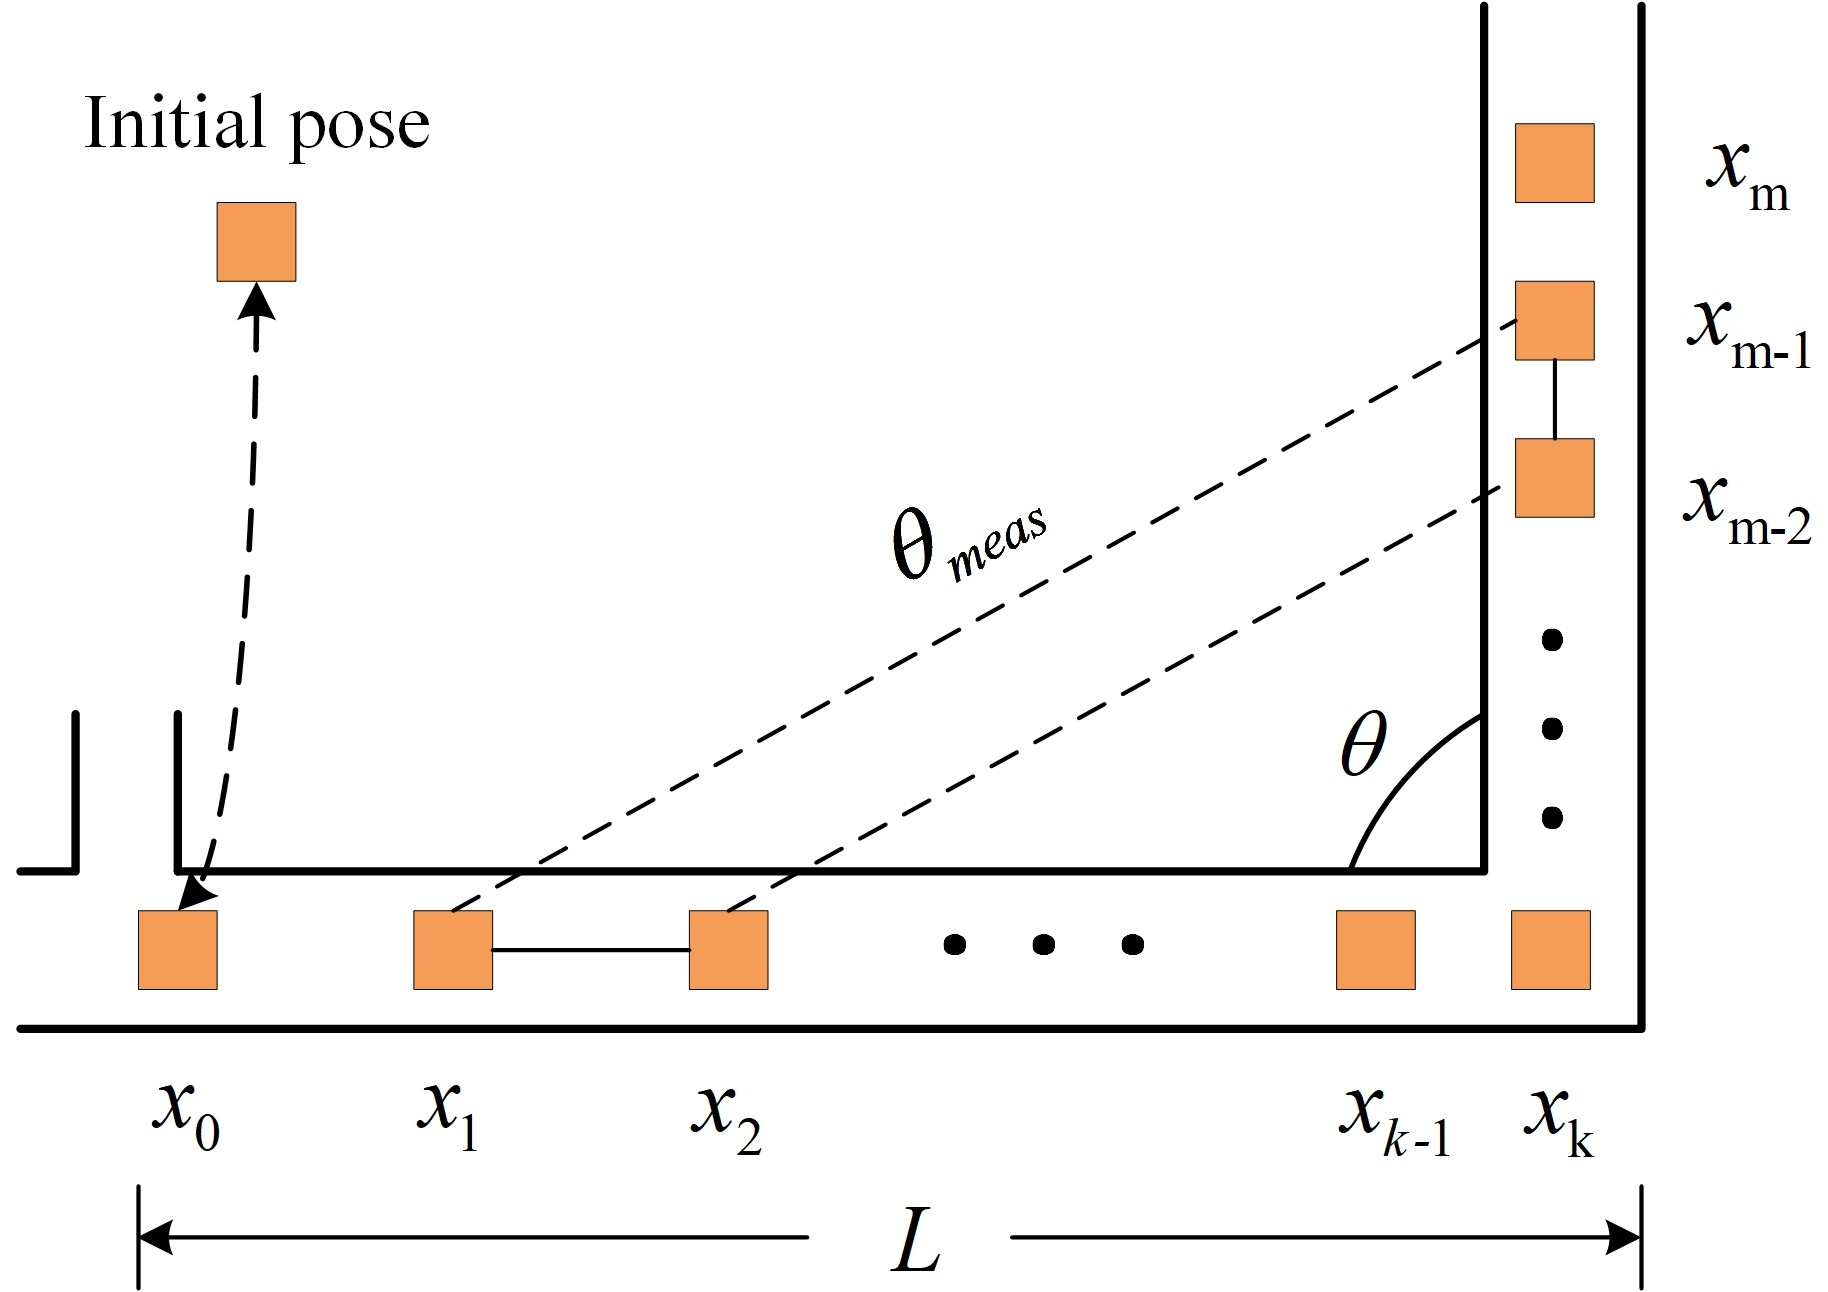
\includegraphics[width=0.88\linewidth]{figures/角度约束-长度约束-修改.jpeg}
    \caption{全局几何先验约束建模示意图}
    \label{fig:global_geom_constraints}
\end{figure}

\subsection{基于轨迹特征拐点选取的长度先验约束}

在矿井巷道场景中，不同巷道段之间通常具有较为明确的结构尺寸信息，例如两处转折区域之间的巷道长度、两段特定结构之间的间距等。与局部帧间位姿约束相比，这类长度信息直接作用于轨迹的全局几何关系，能够有效抑制长距离建图过程中由误差累积引起的结构失真。因此，本文将已知结构长度建模为位姿图中的全局长度约束。

在具体实现中，本文首先通过预设区间的首尾关键帧确定候选巷道段的起止范围，并以首尾关键帧连线作为参考基线。随后，在区间内部计算各关键帧到该基线的平面距离，并结合巷道几何形态确定能够代表结构端点的关键帧；该端点可以是偏离基线最大的转折点，也可以直接取区间起点或终点。如图~\ref{fig:length_constraint} 所示，区间首尾关键帧主要用于限定搜索范围，而长度约束最终作用于两个选定的结构端点之间。

\begin{figure}[htbp]
    \centering
    \resizebox{0.96\linewidth}{!}{
    \begin{tikzpicture}[x=1.15cm,y=1.15cm]
        \draw[rounded corners=2pt, draw=blue!55, fill=blue!8] (0.25,-0.3) rectangle (4.15,1.8);
        \draw[rounded corners=2pt, draw=orange!75, fill=orange!10] (6.0,-0.3) rectangle (9.95,1.8);

        \node[ch3lab] at (2.2,-0.7) {候选区间 1};
        \node[ch3lab] at (7.95,-0.7) {候选区间 2};

        \draw[thick] (0.7,0.15) -- (1.9,0.15) -- (2.9,1.18) -- (3.75,1.18);
        \draw[thick] (6.45,1.08) -- (7.75,1.08) -- (8.75,1.08) -- (9.55,0.35);

        \node[ch3node, label={[ch3lab]below:$s_1$}] (s1) at (0.7,0.15) {};
        \node[ch3node, label={[ch3lab]above:$e_1$}] (e1) at (3.75,1.18) {};
        \node[ch3node, label={[ch3lab]above:$s_2$}] (s2) at (6.45,1.08) {};
        \node[ch3node, label={[ch3lab]below:$e_2$}] (e2) at (9.55,0.35) {};

        \draw[dashed, thin] (s1) -- (e1);
        \draw[dashed, thin] (s2) -- (e2);

        \node[ch3sel, label={[ch3lab]above:$c_1$}] (c1) at (2.9,1.18) {};
        \node[ch3sel, label={[ch3lab]below:$c_2$}] (c2) at (9.55,0.35) {};

        \draw[dashed, gray!70] (c1) -- (2.46,0.78);
        \node[ch3lab, align=center] at (1.55,1.08) {最大偏离\\选转折点};

        \node[ch3lab, align=center] at (8.0,-0.02) {直接选取\\区间端点};
        \node[ch3lab] at (2.25,1.56) {参考基线};
        \node[ch3lab] at (8.0,1.56) {参考基线};

        \draw[dashed, very thick] (c1) -- node[ch3lab, above] {$L^{\mathrm{exp}}$} (c2);
    \end{tikzpicture}}
    \caption{长度约束端点确定与长度先验约束示意图}
    \label{fig:length_constraint}
\end{figure}

设通过上述规则在两个候选区间内分别确定长度约束端点，其对应位姿节点记为 $\mathbf{T}_{c_1}$ 和 $\mathbf{T}_{c_2}$。考虑到巷道长度主要体现在平面结构上，本文采用两节点在 $XY$ 平面内的欧氏距离描述其结构长度，即：
\begin{equation}
d_{c_1,c_2}
=
\left\|
\mathbf{t}_{c_1}^{xy}-\mathbf{t}_{c_2}^{xy}
\right\|_2
\end{equation}

其中，$\mathbf{t}_{c_1}^{xy}$ 和 $\mathbf{t}_{c_2}^{xy}$ 分别表示节点 $\mathbf{T}_{c_1}$ 和 $\mathbf{T}_{c_2}$ 的平面位置向量，$d_{c_1,c_2}$ 为两拐点之间的估计长度。设巷道结构的先验长度为 $L^{\mathrm{exp}}$，则长度约束的误差项可定义为：
\begin{equation}
e_L=d_{c_1,c_2}-L^{\mathrm{exp}}
\end{equation}

由此，对应的长度约束代价项可写为：
\begin{equation}
J_L=e_L^{\mathrm T}\Omega_L e_L
\end{equation}

其中，$\Omega_L$ 为长度约束的信息矩阵，用于描述该先验长度的置信度。通过最小化上述误差，可使优化后的关键帧位置关系尽可能满足已知巷道长度信息。

综上，本节通过在代表性结构端点之间引入长度先验约束，实现了对关键结构相对位置关系的全局补充。

\subsection{基于轨迹段方向的角度先验约束}

除长度信息外，矿井巷道中还普遍存在较为稳定的结构转角关系。例如，不同巷道段之间可能近似正交，或满足已知的夹角先验。相比仅利用局部里程计约束描述相邻帧之间的短程运动关系，转角信息能够直接作用于轨迹段之间的整体方向关系，对抑制累计误差引起的方向偏移具有重要作用。因此，本节进一步构造基于轨迹段方向的角度先验约束，并在后续优化中将其建模为对应因子。

与长度约束直接作用于两个代表性结构点不同，角度约束需要同时描述两段轨迹的方向关系。为此，本文从轨迹中选取四个关键帧节点 $P_1,P_2,P_3,P_4$，其中 $P_1$ 和 $P_2$ 用于确定第一段轨迹方向，$P_3$ 和 $P_4$ 用于确定第二段轨迹方向。对应地，两段轨迹的方向向量可分别表示为：
\begin{equation}
\mathbf{d}_{12}=\mathbf{t}_{P_2}-\mathbf{t}_{P_1}
\end{equation}
\begin{equation}
\mathbf{d}_{34}=\mathbf{t}_{P_4}-\mathbf{t}_{P_3}
\end{equation}

为突出巷道平面结构关系，本文仅考虑轨迹在平面内的方向夹角。于是，两段轨迹之间的实际夹角可表示为：
\begin{equation}
\theta=
\arccos
\left(
\frac{
\mathbf{d}_{12}^{xy}\cdot \mathbf{d}_{34}^{xy}
}{
\|\mathbf{d}_{12}^{xy}\|_2\|\mathbf{d}_{34}^{xy}\|_2
}
\right)
\end{equation}

其中，$\mathbf{d}_{12}^{xy}$ 和 $\mathbf{d}_{34}^{xy}$ 分别表示方向向量在 $XY$ 平面内的投影。设巷道结构的先验夹角为 $\theta^{\mathrm{exp}}$，则角度约束误差可定义为：
\begin{equation}
e_\theta=\theta-\theta^{\mathrm{exp}}
\end{equation}
进一步地，对应的角度约束代价项可表示为：
\begin{equation}
J_\theta=e_\theta^{\mathrm T}\Omega_\theta e_\theta
\end{equation}

其中，$\Omega_\theta$ 为角度约束的信息矩阵，用于描述转角先验的置信度。通过最小化该误差，可使优化后的两段轨迹方向关系尽可能符合巷道结构中的先验夹角信息。
\section{局部几何辅助约束与联合优化}

在完成基础位姿图构建以及全局几何先验约束建模后，本文进一步引入局部结构观测提供的辅助几何信息，对位姿图优化模型进行补充。与全局长度约束和全局角度约束主要描述巷道整体结构关系不同，本节主要考虑两类局部辅助几何约束，即地面平面辅助约束和侧壁方向辅助约束。其中，地面平面辅助约束基于巷道底板在局部范围内通常可近似视为同一平面的假设，为关键帧位姿提供平面参考；侧壁方向辅助约束则利用侧壁方向观测补充转弯区域或局部结构变化区域中的方向信息。两类约束共同用于丰富位姿图中的几何观测信息。

\subsection{基于地面观测的平面辅助约束}

矿井巷道场景中，激光雷达在竖直方向的采样通常相对稀疏；同时，地面点数量通常较少，且激光束与地面的入射角较大，导致地面观测的稳定性和精度相对较弱。因此，关键帧位姿在 $z$ 方向以及俯仰、横滚角上更容易出现误差。另一方面，巷道底板在局部范围内通常具有较稳定的平面结构，可为关键帧位姿估计提供额外的几何参考。为此，本文将地面观测表示为关键帧位姿节点与参考地面平面之间的平面辅助约束关系，并将其纳入后端位姿图优化框架。

在具体建模中，本文将地面引入为全局坐标系中的固定水平参考平面，即：
\begin{equation}
\boldsymbol{\pi}_g=
\begin{bmatrix}
0 & 0 & 1 & 0
\end{bmatrix}^{\mathrm T}
\end{equation}

其中，前三个分量表示平面法向量，最后一个分量表示平面到坐标原点的距离。需要说明的是，本文并不要求真实巷道底板严格为水平面，而是采用固定水平参考平面对关键帧位姿提供辅助约束。该建模方式本质上是一种理想化近似，其主要作用是为 $z$ 方向以及俯仰、横滚角提供稳定参考，而非精确刻画真实底板的几何形态。

对于关键帧 $i$，首先由原始点云提取其对应的局部地面观测。具体而言，点云先根据传感器安装姿态进行俯仰补偿，再依据传感器安装高度和预设高度范围筛选地面候选点，并进一步保留法向接近竖直方向的点；随后采用 RANSAC 对候选点集进行平面拟合，并通过平面法向与竖直方向之间的夹角对拟合结果进行有效性判定。最终，将检测得到的地面平面系数作为关键帧对应的局部地面观测输入后端优化。

【此处建议补图：图 3.x 地面点提取与平面拟合效果图。若后续方便，可展示原始点云、候选地面点以及最终拟合平面内点。相比流程图，这类真实效果图更直观。】

\begin{figure}[htbp]
    \centering
    \begin{tikzpicture}[x=1cm,y=1cm]
        \begin{scope}
            \draw[rounded corners=2pt, thick] (-0.5,-0.6) rectangle (2.7,1.7);
            \foreach \x/\y in {-0.2/0.9,0.1/0.3,0.3/1.1,0.6/0.2,0.9/0.7,1.2/1.0,1.5/0.25,1.8/1.15,2.1/0.55,2.3/1.0,0.0/-0.2,0.4/-0.25,0.8/-0.18,1.2/-0.22,1.6/-0.15,2.0/-0.2} {
                \fill[gray!70] (\x,\y) circle (1.2pt);
            }
            \node[ch3lab] at (1.1,-0.95) {原始点云};
        \end{scope}
        \begin{scope}[xshift=4.2cm]
            \draw[rounded corners=2pt, thick] (-0.5,-0.6) rectangle (2.7,1.7);
            \foreach \x/\y in {-0.2/0.9,0.1/0.3,0.3/1.1,0.6/0.2,0.9/0.7,1.2/1.0,1.5/0.25,1.8/1.15,2.1/0.55,2.3/1.0} {
                \fill[gray!35] (\x,\y) circle (1.2pt);
            }
            \foreach \x/\y in {0.0/-0.2,0.4/-0.25,0.8/-0.18,1.2/-0.22,1.6/-0.15,2.0/-0.2} {
                \fill[green!60!black] (\x,\y) circle (1.4pt);
            }
            \node[ch3lab] at (1.1,-0.95) {候选地面点};
        \end{scope}
        \begin{scope}[xshift=8.4cm]
            \draw[rounded corners=2pt, thick] (-0.5,-0.6) rectangle (2.7,1.7);
            \draw[very thick, blue!70] (-0.2,-0.28) -- (2.3,-0.08);
            \foreach \x/\y in {0.0/-0.2,0.4/-0.25,0.8/-0.18,1.2/-0.22,1.6/-0.15,2.0/-0.2} {
                \fill[green!60!black] (\x,\y) circle (1.4pt);
            }
            \node[ch3lab] at (1.1,-0.95) {RANSAC 平面拟合};
        \end{scope}
        \draw[ch3arr] (2.95,0.55) -- (3.75,0.55);
        \draw[ch3arr] (7.15,0.55) -- (7.95,0.55);
    \end{tikzpicture}
    \caption{地面点提取与平面拟合示意图}
    \label{fig:floor_extraction_pipeline}
\end{figure}

设关键帧 $i$ 对应的局部地面观测平面为：
\begin{equation}
\boldsymbol{\pi}_i=
\begin{bmatrix}
\mathbf{n}_i\\
d_i
\end{bmatrix}
\end{equation}

其中，$\mathbf{n}_i$ 为局部地面平面的单位法向量，$d_i$ 为平面到局部坐标系原点的距离。设关键帧位姿为 $\mathbf{T}_i=[\mathbf{R}_i \mid \mathbf{t}_i]$，则参考地面平面在关键帧局部坐标系下的表示可记为 $\boldsymbol{\pi}_g^l$。参考 HDL-Graph-SLAM 的处理方式，可将参考平面在局部坐标系中的参数表示为：
\begin{equation}
\mathbf{n}_g^{l}=\mathbf{R}_i^{\mathrm T}\mathbf{n}_g
\end{equation}
\begin{equation}
d_g^{l}=d_g-\mathbf{t}_i^{\mathrm T}\mathbf{n}_g^{l}
\end{equation}

其中，$\mathbf{n}_g$ 和 $d_g$ 分别为全局参考地面平面的法向量和距离参数。

由于三维平面仅具有 $3$ 个自由度，而 Hessian 形式属于带单位法向约束的 $4$ 维过参数化表示，若直接用于优化建模会引入参数冗余。为便于构造低维残差项，本文借鉴 CPA-SLAM\cite{Ma2016CPASLAM} 中的处理方式，采用平面的最小参数化表示：
\begin{equation}
\tau(\boldsymbol{\pi})=(\phi,\psi,d)
\end{equation}
其中，$\phi$ 和 $\psi$ 用于描述平面法向方向，$d$ 为平面到坐标原点的距离参数。采用该表示后，关键帧位姿节点与参考地面平面之间的残差可定义为：
\begin{equation}
\mathbf{e}_{g,i}
=
\tau(\boldsymbol{\pi}_g^l)-\tau(\boldsymbol{\pi}_i)
\end{equation}
对应的代价项可表示为：
\begin{equation}
J_{g,i}
=
\mathbf{e}_{g,i}^{\mathrm T}
\boldsymbol{\Omega}_{g,i}
\mathbf{e}_{g,i}
\end{equation}

其中，$\boldsymbol{\Omega}_{g,i}$ 为地面辅助约束的信息矩阵，用于描述该观测的置信度。通过最小化该误差，可使优化后的关键帧位姿在局部范围内更符合地面观测提供的平面参考。

从作用机理上看，该平面辅助约束能够在一定程度上减弱关键帧位姿在垂直方向和姿态上的漂移，尤其在场景地面较平整、局部观测较稳定时，可为图优化提供额外的几何支撑。然而需要指出的是，本文采用的固定水平参考平面仅是一种理想化近似，真实巷道底板可能存在坡度或局部起伏，因此该约束与真实场景之间不可避免地存在模型失配。当坡度变化较小或局部起伏不明显时，该约束能够有效抑制 $z$ 方向漂移；而当地面起伏较大时，其作用会受到限制。因此，本文将地面约束定位为辅助几何约束，而非用于精确描述底板几何形态的核心约束。

【此处建议补图：图 3.x 地面平面辅助约束示意图。建议画法为：一个关键帧局部坐标系、一块由点云拟合得到的局部地面平面，以及一个全局水平参考平面，并用箭头表示参考平面经位姿变换后与局部观测平面建立残差关系。该图较好画，也能直接体现“理想水平平面假设”。】

\begin{figure}[htbp]
    \centering
    \resizebox{0.92\linewidth}{!}{
    \begin{tikzpicture}[x=1cm,y=1cm, >=Latex]
        % global frame and reference plane
        \draw[thick, ->] (0,0) -- (0,2.2) node[left] {$z_g$};
        \draw[thick, ->] (0,0) -- (2.5,0) node[below] {$x_g$};
        \coordinate (ga) at (-0.35,0.78);
        \coordinate (gb) at (1.95,0.78);
        \coordinate (gc) at (2.45,1.18);
        \coordinate (gd) at (0.15,1.18);
        \filldraw[fill=blue!12, draw=blue!70!black, thick] (ga) -- (gb) -- (gc) -- (gd) -- cycle;
        \draw[blue!70!black, very thick, ->] (1.1,0.98) -- +(0,0.95) node[right] {$\mathbf{n}_g$};
        \node[ch3lab, blue!70!black] at (1.05,1.48) {全局参考平面 $\boldsymbol{\pi}_g$};

        % transform arrow
        \draw[ch3arr] (3.05,1.12) -- node[ch3lab, above] {$\mathbf{T}_i$} (5.25,1.12);

        % local frame and planes
        \begin{scope}[shift={(6.2,0.15)}, rotate=12]
            \draw[thick, ->] (0,0) -- (0,2.0) node[left] {$z_i$};
            \draw[thick, ->] (0,0) -- (2.4,0) node[below] {$x_i$};

            % transformed reference plane in local frame
            \coordinate (ra) at (-0.25,0.82);
            \coordinate (rb) at (2.00,0.82);
            \coordinate (rc) at (2.45,1.18);
            \coordinate (rd) at (0.20,1.18);
            \filldraw[fill=blue!8, draw=blue!70!black, dashed, thick] (ra) -- (rb) -- (rc) -- (rd) -- cycle;
            \draw[blue!70!black, thick, dashed, ->] (1.1,1.00) -- +(0,0.82);

            % observed local ground plane
            \coordinate (la) at (-0.05,0.58);
            \coordinate (lb) at (2.20,0.72);
            \coordinate (lc) at (2.60,1.08);
            \coordinate (ld) at (0.35,0.94);
            \filldraw[fill=orange!18, draw=orange!80!black, thick] (la) -- (lb) -- (lc) -- (ld) -- cycle;
            \draw[orange!80!black, very thick, ->] (1.35,0.82) -- +(-0.12,0.88);

            % keyframe origin
            \fill[black] (0,0) circle (1.1pt);
            \node[ch3lab] at (0.28,-0.25) {关键帧 $i$};

            % residual
            \draw[ch3darr, red!70!black] (1.72,1.28) -- +(0.0,-0.42);
            \node[ch3lab, red!70!black] at (2.15,1.08) {$\mathbf{e}_{g,i}$};
            \node[ch3lab, blue!70!black] at (2.18,1.56) {$\boldsymbol{\pi}_g^{l}$};
            \node[ch3lab, orange!80!black] at (2.55,0.42) {$\boldsymbol{\pi}_i$};
        \end{scope}
    \end{tikzpicture}}
    \caption{地面平面辅助约束示意图}
    \label{fig:ground_pose_plane_constraint}
\end{figure}

【此处建议后续补表：表 3.x 地面与侧壁观测相关参数设置。可列出地面提取与侧壁提取所用的高度范围、法线阈值、RANSAC 距离阈值、最小内点数等参数。】

\subsection{基于侧壁观测的方向辅助约束}

除地面外，巷道侧壁同样包含较为稳定的局部结构信息。尤其在转弯区域，先前墙段与当前墙段之间往往具有较明确的方向关系，因此可进一步利用侧壁观测构造局部辅助约束。

侧壁观测的提取过程与 3.4.1 节中地面平面观测的提取方法类似，同样通过候选点筛选、RANSAC 平面分割和有效性判定获得局部平面观测。不同之处在于，侧壁提取主要在预设侧向区域内进行，并结合平面法向方向和相邻帧稳定性对检测结果进行筛选。经筛选后的侧壁平面参数被用于表征当前关键帧附近的局部结构方向。

设任意关键帧 $k$ 在局部坐标系下提取的侧壁方向观测为 $\mathbf{n}_k^{l}$。为便于不同关键帧之间的方向比较，首先利用关键帧姿态的旋转部分将其统一变换到全局坐标系下，即：
\begin{equation}
\mathbf{n}_k=\mathbf{R}_k\mathbf{n}_k^{l}
\end{equation}

为减弱单帧观测噪声的影响，本文先在历史轨迹中选取一段连续的有效侧壁观测：
\begin{equation}
\mathcal{S}_j=\{j-r,\ldots,j\}
\end{equation}

并对该段观测对应的侧壁方向进行累计与归一化，从而得到先前墙段的代表方向：
\begin{equation}
\bar{\mathbf{n}}_j=
\frac{\sum_{k\in\mathcal{S}_j}\mathbf{n}_k}
{\left\|\sum_{k\in\mathcal{S}_j}\mathbf{n}_k\right\|_2}
\end{equation}

当当前关键帧 $i$ 检测到有效侧壁方向观测 $\mathbf{n}_i$，且该观测与先前墙段可能构成局部转角关系时，才进一步构造侧壁方向辅助约束。其示意如图~\ref{fig:sidewall_aux_constraint} 所示。其中，$\bar{\mathbf{n}}_j$ 表示由历史墙段观测形成的代表方向，$\mathbf{n}_i$ 表示当前关键帧的侧壁方向观测。

设先前墙段代表方向与当前侧壁方向之间的夹角为 $\phi_{j,i}$，则有：
\begin{equation}
\phi_{j,i}=
\arccos
\left(
\frac{
\bar{\mathbf{n}}_j^{\mathrm T}\mathbf{n}_i
}{
\|\bar{\mathbf{n}}_j\|_2\|\mathbf{n}_i\|_2
}
\right)
\end{equation}

设局部结构对应的先验夹角为 $\phi_{j,i}^{\mathrm{exp}}$，则对应残差可定义为：
\begin{equation}
e_{w,j,i}=\phi_{j,i}-\phi_{j,i}^{\mathrm{exp}}
\end{equation}

相应的代价项可表示为：
\begin{equation}
J_{w,j,i}=e_{w,j,i}^{\mathrm T}\Omega_{w,j,i}e_{w,j,i}
\end{equation}

其中，$\Omega_{w,j,i}$ 为侧壁方向辅助约束的信息矩阵。仅当当前观测与先前墙段满足候选角关系时，才将该约束接入优化。

\begin{figure}[htbp]
    \centering
    \resizebox{0.96\linewidth}{!}{
    \begin{tikzpicture}[x=1cm,y=1cm, >=Latex]
        % left panel
        \fill[blue!4, rounded corners=5pt] (-0.6,-0.95) rectangle (5.55,3.05);
        \draw[rounded corners=5pt, thick, gray!70] (-0.6,-0.95) rectangle (5.55,3.05);
        \node[ch3lab, font=\small\bfseries] at (2.48,2.75) {先前墙段观测集合 $\mathcal{S}_j$};

        % corridor walls
        \draw[line width=1.1pt, gray!65] (-0.05,0.25) -- (1.15,0.34) -- (2.35,0.24) -- (3.55,0.36) -- (4.8,0.28);
        \draw[line width=1.1pt, gray!65] (0.25,1.65) -- (1.45,1.74) -- (2.65,1.64) -- (3.85,1.76) -- (5.1,1.68);
        \draw[dashed, gray!55] (0.1,0.95) -- (1.3,1.04) -- (2.5,0.94) -- (3.7,1.06) -- (4.95,0.98);

        \foreach \x/\y/\lab in {0.55/0.98/$K_{j-r}$,1.75/1.07/$K_{j-r+1}$,2.95/0.98/$\cdots$,4.15/1.10/$K_j$} {
            \node[ch3node, label={[ch3lab]below:\lab}] at (\x,\y) {};
        }

        \draw[very thick, blue!60!black,-{Latex[length=2.4mm]}] (0.45,1.15) -- ++(0.92,0.07);
        \draw[very thick, blue!60!black,-{Latex[length=2.4mm]}] (1.65,1.24) -- ++(0.88,-0.02);
        \draw[very thick, blue!60!black,-{Latex[length=2.4mm]}] (2.85,1.14) -- ++(0.92,0.08);
        \draw[very thick, blue!60!black,-{Latex[length=2.4mm]}] (4.0,1.26) -- ++(0.86,-0.01);
        \node[ch3lab, blue!60!black] at (1.25,1.55) {$\mathbf{n}_k$};

        \draw[rounded corners=3pt, fill=white, draw=blue!35] (3.1,2.0) rectangle (5.15,2.55);
        \node[ch3lab, align=center] at (4.12,2.27) {累计与归一化\\形成代表方向};

        \coordinate (histref) at (4.45,0.45);
        \draw[very thick, red!75!black,-{Latex[length=2.6mm]}] (histref) -- ++(0.85,1.22);
        \node[ch3lab, red!75!black] at (5.0,1.85) {$\bar{\mathbf{n}}_j$};

        % bridge arrow
        \draw[ch3arr, thick] (5.95,1.03) -- node[ch3lab, above, align=center] {满足候选角关系\\后接入约束} (7.35,1.03);

        % right panel
        \fill[orange!4, rounded corners=5pt] (7.65,-0.95) rectangle (14.0,3.05);
        \draw[rounded corners=5pt, thick, gray!70] (7.65,-0.95) rectangle (14.0,3.05);
        \node[ch3lab, font=\small\bfseries] at (10.82,2.75) {当前帧局部墙面观测与约束构造};

        % local wall geometry
        \draw[line width=1.2pt, orange!55!black] (8.25,0.10) -- (9.45,0.48) -- (10.85,1.78);
        \draw[line width=1.2pt, orange!55!black] (8.65,-0.35) -- (9.9,0.08) -- (11.28,1.35);
        \draw[dashed, gray!55] (8.45,-0.12) -- (9.68,0.28) -- (11.05,1.56);

        \node[ch3node, fill=orange!18, draw=orange!80!black, label={[ch3lab]below:$K_i$}] (cur) at (9.7,0.28) {};

        \draw[very thick, orange!85!black,-{Latex[length=2.6mm]}] (cur) -- ++(1.05,0.35);
        \node[ch3lab, orange!85!black] at (11.05,0.42) {$\mathbf{n}_i$};

        \draw[very thick, red!75!black,-{Latex[length=2.6mm]}] (cur) -- ++(0.72,1.12);
        \node[ch3lab, red!75!black] at (10.8,1.62) {$\bar{\mathbf{n}}_j$};

        \draw[thick] ($(cur)+(0.78,0.18)$) arc[start angle=18,end angle=57,radius=0.82];
        \node[ch3lab] at (10.43,1.0) {$\phi_{j,i}$};

        \draw[rounded corners=3pt, fill=white, draw=red!35] (12.05,0.1) rectangle (13.55,1.58);
        \node[ch3lab, align=center] at (12.8,0.95) {残差构造\\$e_{w,j,i}=\phi_{j,i}-\phi_{j,i}^{\mathrm{exp}}$};

        \node[ch3lab, align=center] at (9.1,-0.62) {当前帧检测到有效墙面方向};
        \node[ch3lab, align=center] at (4.65,-0.62) {历史墙段提供局部代表方向};
    \end{tikzpicture}}
    \caption{侧壁方向辅助约束示意图}
    \label{fig:sidewall_aux_constraint}
\end{figure}

\subsection{多因子联合优化模型与求解}

前文构建的基础位姿图、全局几何先验约束以及局部辅助几何约束，均可统一纳入同一因子图优化框架。具体而言，关键帧位姿作为变量节点，里程计约束、长度约束、角度约束、地面平面辅助约束和侧壁方向辅助约束分别作为不同类型的因子接入图模型，并共同作用于同一组状态变量。下面给出本文多因子联合优化模型及其求解形式。

设位姿图中所有关键帧状态变量集合为：
\begin{equation}
\mathcal{X}=\{\mathbf{T}_1,\mathbf{T}_2,\cdots,\mathbf{T}_N\}
\end{equation}

则整体优化目标可表示为各类约束代价项的加权和，即：
\begin{equation}
\min_{\mathcal{X}}
\left(
\sum_{(i-1,i)\in\mathcal{E}_o}J_{o,i}
+
\sum_{l\in\mathcal{E}_L}J_{L,l}
+
\sum_{a\in\mathcal{E}_\theta}J_{\theta,a}
+
\sum_{g\in\mathcal{E}_g}J_{g,g}
+
\sum_{w\in\mathcal{E}_w}J_{w,w}
\right)
\end{equation}

在各类观测误差局部近似服从高斯分布的条件下，本文对各类因子统一采用加权二次型残差进行建模，其中信息矩阵 $\boldsymbol{\Omega}$ 可视为对应协方差矩阵的逆，用于刻画不同约束的置信度与权重分配。

其中，$\mathcal{E}_o$、$\mathcal{E}_L$、$\mathcal{E}_\theta$、$\mathcal{E}_g$ 和 $\mathcal{E}_w$ 分别表示里程计约束集合、长度约束集合、角度约束集合、地面约束集合和侧壁约束集合；$J_{o,i}$、$J_{L,l}$、$J_{\theta,a}$、$J_{g,g}$ 和 $J_{w,w}$ 分别表示对应约束项的代价函数。

上述优化问题可进一步写成非线性最小二乘形式。求解时，以基础位姿图给出的关键帧初始位姿作为初值，对目标函数在当前估计处进行线性化，并利用稀疏矩阵结构进行迭代求解。为提高优化鲁棒性，对于全局长度约束和全局角度约束等先验因子，可进一步引入鲁棒核函数，以减弱异常约束对最终结果的影响。最终得到优化后的关键帧位姿，并据此更新地图结果。

【此处建议补图：图 3.x 多因子联合优化模型示意图。建议画法为：中间是一串关键帧节点及相邻里程计边；上方跨节点连接长度约束和角度约束；下方或侧边连接地面约束和侧壁约束；最后统一指向“图优化求解”模块。该图很好画，也适合作为 3.4 节的总结图。】

\begin{figure}[htbp]
    \centering
    \begin{tikzpicture}[x=1.5cm,y=1cm]
        \foreach \i/\y in {0/0.0,1/0.18,2/-0.05,3/0.22,4/0.05} {
            \node[ch3node, label={[ch3lab]below:$\mathbf{T}_{\i+1}$}] (n\i) at (\i,\y) {};
        }
        \draw[thick] (n0) -- (n1) -- (n2) -- (n3) -- (n4);
        \node[ch3lab] at (2,-0.6) {里程计约束};

        \draw[orange!80!black, very thick, dashed] (n1) to[bend left=30] node[ch3lab, above] {长度约束} (n3);
        \draw[red!70!black, very thick, dashed] (n0) to[bend left=48] node[ch3lab, above] {角度约束} (n4);

        \node[ch3aux, below=10mm of n1] (g1) {地面约束};
        \node[ch3aux, below=10mm of n3] (w1) {侧壁约束};
        \draw[ch3darr] (g1) -- (n1);
        \draw[ch3darr] (w1) -- (n3);

        \node[ch3solve, right=18mm of n4] (solver2) {统一图优化};
        \draw[ch3arr] (n4) -- (solver2);
        \draw[ch3arr] (g1.east) -| (solver2.south);
        \draw[ch3arr] (w1.east) -| (solver2.south);
    \end{tikzpicture}
    \caption{多因子联合优化模型示意图}
    \label{fig:joint_factor_graph}
\end{figure}

【此处建议补表：表 3.x 多因子约束汇总表。建议列出“约束名称—作用对象—误差形式—约束作用—核心/辅助属性”。这张表很有用，尤其适合放在本小节末尾。】

\section{实验验证}

为验证本文所提出的基于几何结构约束的矿井巷道建图方法的有效性，本文分别在公开 Bruceton Mine 数据集、真实地下矿井数据集和 Gazebo 仿真数据集上开展实验验证。

\subsection{数据集说明}

本文实验采用公开 Bruceton Mine 数据集、真实地下矿井数据集和 Gazebo 仿真数据集。

（1）Bruceton Mine 数据集

Bruceton Mine 数据集由 Reinke 等人发布，对应数据采集地点为美国宾夕法尼亚州匹兹堡的 Bruceton Research Mine（布鲁斯顿矿井）。该数据集采用 Husky 机器人作为移动平台，搭载 3 个完成外参标定的 VLP-16 激光雷达，扫描频率为 10 Hz。与本文单雷达建图设置一致，实验中选取 3 个激光雷达中水平安装的单个雷达数据作为输入。

在数据序列选择上，本文从原始数据中截取了一段长度为 352.82 m、包含长直巷道的轨迹作为实验对象。该序列场景重复性较强、回环信息较少，适合用于评估所提方法在地下矿井长走廊环境中的累计误差抑制能力。

\begin{figure}[htbp]
    \centering
    \begin{tikzpicture}
        \node[draw, rounded corners=4pt, thick, minimum width=13cm, minimum height=4.8cm, align=center, fill=gray!8, text width=11.2cm] {
            此处插入 Bruceton Mine 数据集典型场景图\\[4pt]
            建议展示形式：点云俯视图、场景截图或巷道结构示意图。
        };
    \end{tikzpicture}
    \caption{Bruceton Mine 数据集典型场景}
    \label{fig:bruceton_scene}
\end{figure}

（2）真实地下矿井数据集

真实地下矿井数据集采集于陕西大海则煤矿井下巷道，由地面移动机器人搭载 Ouster OS1-128 激光雷达完成数据采集，采样频率为 10 Hz，整个采集轨迹长度为 1641.81 m，采集时长为 11.47 min。该数据集具有巷道狭长、结构重复和长距离连续延伸等特点，可用于检验本文方法在真实矿井场景中的适用性。本文采用人工后处理构建的高精度参考地图，并在该参考地图上通过独立的实时定位流程生成参考轨迹，用于后续结果对比与误差评估。实验中同时从轨迹整体形态和参考轨迹误差两个方面对建图结果进行比较。

\begin{figure}[htbp]
    \centering
    \begin{tikzpicture}
        \node[draw, rounded corners=4pt, thick, minimum width=13cm, minimum height=4.8cm, align=center, fill=gray!8, text width=11.2cm] {
            此处插入真实地下矿井数据集典型场景图\\[4pt]
            建议展示形式：陕西大海则煤矿井下巷道现场照片、点云强度图或巷道截面图。
        };
    \end{tikzpicture}
    \caption{真实地下矿井数据集典型场景}
    \label{fig:realmine_scene}
\end{figure}

（3）Gazebo 仿真数据集

Gazebo 仿真数据集由本文构建的巷道仿真环境生成。仿真平台采用四轮移动机器人模型，搭载参考 Ouster OS1-64 配置的 64 线激光雷达仿真模型，扫描频率为 10 Hz，实验轨迹长度约为 142.00 m。该仿真雷达模型在量测距离中叠加高斯噪声，并通过将机器人模型位姿与激光雷达时间戳对齐获得真值轨迹。该数据集主要用于在可控场景下补充验证所提几何结构约束的作用机理，并为后续误差分析提供精确参考。

\begin{figure}[htbp]
    \centering
    \begin{tikzpicture}
        \node[draw, rounded corners=4pt, thick, minimum width=13cm, minimum height=4.8cm, align=center, fill=gray!8, text width=11.2cm] {
            此处插入 Gazebo 仿真数据集典型场景图\\[4pt]
            建议展示形式：仿真巷道俯视图、机器人运行截图或场景结构示意图。
        };
    \end{tikzpicture}
    \caption{Gazebo 仿真数据集典型场景}
    \label{fig:gazebo_scene}
\end{figure}

\subsection{对比方法与实验结果分析}

当前主流开源激光建图方法包括 LOAM、LeGO-LOAM、Cartographer 和 HDL-Graph-SLAM 等。其中，LOAM 与 LeGO-LOAM 均适用于三维激光雷达建图，LeGO-LOAM 是在 LOAM 基础上的改进方法；Cartographer 采用子图优化框架，在二维激光建图中应用较为广泛，但其三维建图流程与本文基于关键帧位姿图和几何约束的建模方式差异较大；HDL-Graph-SLAM 同样面向三维激光雷达，并采用图优化框架引入地面等约束。考虑到本文研究的是三维激光雷达矿井巷道建图问题，本文选取 LeGO-LOAM 和 HDL-Graph-SLAM 作为对比方法。评价指标采用第 2 章所述绝对误差指标。

为了比较不同方法的建图性能，本文分别对 Bruceton Mine 数据集、真实地下矿井数据集和 Gazebo 仿真数据集上的估计轨迹进行分析。图~\ref{fig:bruceton_traj_compare}、图~\ref{fig:realmine_traj_compare} 和图~\ref{fig:gazebo_traj_compare} 分别给出了 3 个数据集下不同算法的轨迹或地图对比结果。其中，黑色虚线表示参考轨迹或参考地图，橙色实线表示 LeGO-LOAM 的估计结果，蓝绿色实线表示 HDL-Graph-SLAM 的估计结果，红色实线表示本文方法的估计结果。

\begin{figure}[htbp]
    \centering
    \begin{tikzpicture}[x=1cm,y=1cm]
        \foreach \x/\name in {0/LeGO-LOAM,4.3/HDL-Graph-SLAM,8.6/本文方法} {
            \draw[rounded corners=3pt, thick] (\x,0) rectangle ++(3.6,3.1);
            \node[ch3lab] at (\x+1.8,3.35) {\name};
        }

        \draw[black, thick] (0.25,0.55) -- (1.20,0.85) -- (2.45,0.85) -- (3.20,2.45);
        \draw[orange!85!black, very thick] (0.25,0.55) -- (1.35,0.95) -- (2.55,1.12) -- (3.00,2.75);

        \draw[black, thick] (4.55,0.55) -- (5.50,0.85) -- (6.75,0.85) -- (7.50,2.45);
        \draw[teal!70!black, very thick] (4.55,0.55) -- (5.55,0.90) -- (6.90,1.08) -- (7.22,2.82);

        \draw[black, thick] (8.85,0.55) -- (9.80,0.85) -- (11.05,0.85) -- (11.80,2.45);
        \draw[red!75!black, very thick] (8.85,0.55) -- (9.78,0.82) -- (11.02,0.88) -- (11.78,2.50);

        \node[ch3lab] at (6.0,-0.45) {黑色为参考轨迹，彩色为各方法估计轨迹；后续可替换为真实实验图};
    \end{tikzpicture}
    \caption{Bruceton Mine 数据集上的轨迹对比结果}
    \label{fig:bruceton_traj_compare}
\end{figure}

图~\ref{fig:realmine_traj_compare} 建议展示不同方法在真实地下矿井场景中的轨迹或建图结果对比，可采用“全局地图叠加轨迹”或“局部典型区域放大图”的形式进行呈现。建议重点突出长直巷道、转弯连接区域以及结构重复区域的差异，从而更直观地体现本文方法在全局一致性和局部结构保持方面的优势。

\begin{figure}[htbp]
    \centering
    \begin{tikzpicture}
        \node[draw, rounded corners=4pt, thick, minimum width=13cm, minimum height=5.2cm, align=center, fill=gray!8, text width=11.3cm] {
            此处插入真实地下矿井数据集轨迹/地图对比图\\[4pt]
            建议展示形式：参考轨迹与不同方法轨迹的俯视叠加图，\\[2pt]
            或者全局点云地图与优化后轨迹的叠加图。\\[4pt]
            建议重点标出长直巷道段、转弯处以及易发生漂移的典型区域。
        };
    \end{tikzpicture}
    \caption{真实地下矿井数据集上的轨迹或地图对比结果}
    \label{fig:realmine_traj_compare}
\end{figure}

图~\ref{fig:gazebo_traj_compare} 建议展示 Gazebo 仿真数据集上的轨迹或建图结果对比，可采用“真值轨迹与估计轨迹俯视叠加图”或“仿真地图与优化后轨迹叠加图”的形式进行呈现。

\begin{figure}[htbp]
    \centering
    \begin{tikzpicture}
        \node[draw, rounded corners=4pt, thick, minimum width=13cm, minimum height=5.0cm, align=center, fill=gray!8, text width=11.3cm] {
            此处插入 Gazebo 仿真数据集轨迹/地图对比图\\[4pt]
            建议展示形式：真值轨迹与不同方法轨迹的俯视叠加图，\\[2pt]
            或者仿真场景地图与优化后轨迹的叠加图。\\[4pt]
            建议重点标出长直巷道段、转弯处以及结构约束起作用的典型区域。
        };
    \end{tikzpicture}
    \caption{Gazebo 仿真数据集上的轨迹或地图对比结果}
    \label{fig:gazebo_traj_compare}
\end{figure}

从 3 个数据集的对比结果来看，在 Bruceton Mine 数据集的长直巷道场景下，LeGO-LOAM 和 HDL-Graph-SLAM 均会出现不同程度的轨迹偏移与累计误差，而本文方法的估计轨迹与参考轨迹更加接近；在真实地下矿井数据集上，本文方法在长距离连续建图过程中能够较好地保持巷道结构的整体形态，并在结构重复区域表现出更稳定的建图结果；在 Gazebo 仿真数据集上，依托精确真值轨迹可进一步验证所提几何结构约束在规则巷道场景中的作用。各数据集的定量结果统一汇总于表~\ref{tab:result_summary}，其中 Bruceton Mine 数据集已经给出了本文方法与 HDL-Graph-SLAM 的均方根误差和平均数结果，中位数以及其余数据集的数值可在后续实验完成后继续补入。

\begin{table}[htbp]
    \centering
    \caption{各数据集的定量对比结果}
    \label{tab:result_summary}
    \small
    \begin{tabular}{ccccc}
        \toprule
        数据集 & 算法 & \shortstack{均方根误差\\(m)} & \shortstack{平均数\\(m)} & \shortstack{中位数\\(m)} \\
        \midrule
        \multirow{3}{*}{Bruceton Mine 数据集} & LeGO-LOAM & 待补充 & 待补充 & 待补充 \\
         & HDL-Graph-SLAM & 1.39 & 1.13 & 待补充 \\
         & 本文方法 & 0.25 & 0.20 & 待补充 \\
        \multirow{3}{*}{真实地下矿井数据集} & LeGO-LOAM & 待补充 & 待补充 & 待补充 \\
         & HDL-Graph-SLAM & 待补充 & 待补充 & 待补充 \\
         & 本文方法 & 待补充 & 待补充 & 待补充 \\
        \multirow{3}{*}{Gazebo 仿真数据集} & LeGO-LOAM & 待补充 & 待补充 & 待补充 \\
         & HDL-Graph-SLAM & 待补充 & 待补充 & 待补充 \\
         & 本文方法 & 待补充 & 待补充 & 待补充 \\
        \bottomrule
    \end{tabular}
\end{table}

\subsection{实验结果讨论}

综合当前各数据集的实验结果可以看出，本文方法在矿井巷道场景中具有较好的适用性。对于公开 Bruceton Mine 数据集，所引入的全局长度约束和全局角度约束能够有效抑制长距离运行中的误差累积，并显著提升轨迹精度；对于真实地下矿井数据集，所提方法能够在复杂工程环境下保持较好的地图结构一致性；Gazebo 仿真数据集则可作为补充验证场景，用于进一步分析所提几何结构约束的作用机理。

总体而言，本文方法的优势主要体现在以下两个方面：其一，能够充分利用矿井巷道场景中客观存在的几何结构先验，将传统仅依赖局部配准的建图问题扩展为融合全局结构信息的图优化问题；其二，在真实场景中，当局部观测受退化、遮挡或重复结构影响时，几何约束仍可为位姿优化提供补充信息，从而提高建图结果的稳定性。后续在补充真实矿井数据的详细定量结果后，可进一步从局部典型区域、误差统计分布以及消融实验等角度展开更深入的分析。

\section{本章小结}

本章围绕矿井巷道场景中长距离建图易产生累计漂移和全局一致性不足的问题，提出了一种基于几何结构约束的位姿图建图方法。首先，本文以关键帧位姿为状态变量，构建了包含时间关联、关键帧筛选和里程计边的基础位姿图模型；随后，针对矿井巷道场景中普遍存在的结构规律，分别建立了基于代表性拐点的全局长度约束和基于轨迹段方向关系的全局角度约束，用于从全局尺度抑制轨迹漂移；在此基础上，进一步引入地面平面辅助约束和侧壁方向辅助约束，以增强局部区域的几何表达能力，并构建了统一的多因子联合优化模型。

实验结果表明，本文方法在公开 Bruceton Mine 数据集、真实地下矿井数据集以及 Gazebo 仿真数据集上均表现出较好的适用性，并在长距离运行条件下体现出更优的轨迹一致性和误差控制能力。尤其是在长直巷道和结构重复区域，引入几何结构先验后，轨迹累计误差得到有效抑制，验证了所提方法的有效性和工程应用潜力。下一章将在此基础上进一步研究矿井巷道场景中的定位问题，探讨如何利用先验地图和几何约束提升定位精度与鲁棒性。
